\documentclass[a4paper,12pt,twoside,openany]{book}
\usepackage{amd}
\usepackage{framed}
\usepackage{mathrsfs}

% %--------------------------------------------------------------------------
% %         General Setting
% %--------------------------------------------------------------------------

\graphicspath{{Images/}{../Images/}} %Path of figures
\setkeys{Gin}{width=0.85\textwidth} %Size of figures
\setlength{\cftbeforechapskip}{3pt} %space between items in toc
\setlength{\parindent}{0.5cm} % Idk
% Theorem System
% The following boxes are provided:
%   Definition:     \defn 
%   Theorem:        \thm 
%   Lemma:          \lem
%   Corollary:      \cor
%   Proposition:    \prop   
%   Claim:          \clm
%   Fact:           \fact
%   Proof:          \pf
%   Example:        \ex
%   Remark:         \rmk (sentence), \rmkb (block)
% Suffix
%   r:              Allow Theorem/Definition to be referenced, e.g. thmr
%   p:              Add a short proof block for Lemma, Corollary, Proposition or Claim, e.g. lemp
%                   For theorems, use \pf for proof blocks

% ======= Real examples : 

% \defn{Definition Name}{
%     A defintion.
% }

% \thmr{Theorem Name}{mybigthm}{
%     A theorem.
% }

% \lem{Lemma Name}{
%     A lemma.
% }

% \fact{
%     A fact.
% }

% \cor{
%     A corollary.
% }

% \prop{
%     A proposition.
% }

% \clmp{}{
%     A claim.
% }{
%     A reference to Theorem~\ref{thm:mybigthm}
% }

% \pf{
%    proof.

% \ex{
%     some examples. 
% }

% \rmk{
%     Some remark.
% }

% \rmkb{
%     Some more remark.
% }

\usepackage{xcolor}

% Define custom colors
\definecolor{defscol}{HTML}{ecd8d7} %For definitions
\definecolor{asumscol}{HTML}{ecd8d7} %For Assumptions

\definecolor{rmkscol}{HTML}{313160} %For remarks
\definecolor{exmscol}{HTML}{e04b52} %For examples

\definecolor{lemscol}{HTML}{2c3943} %For Lemmes
\definecolor{thmscol}{HTML}{595765} %For Theorems
\definecolor{prpscol}{HTML}{9c98b1} %For proposition
\definecolor{corscol}{HTML}{dfd9fd} %For corrolaries

\definecolor{clmscol}{HTML}{165c58} %For claims
\definecolor{facscol}{HTML}{28a8a1} %For facts



% ============================
% Definition
% ============================
\newtcbtheorem[number within=section]{mydefinition}{Definition}
{
    enhanced,
    frame hidden,
    titlerule=0mm,
    toptitle=1mm,
    bottomtitle=1mm,
    fonttitle=\bfseries\large,
    coltitle=black,
    colbacktitle=defscol!40!white,
    colback=defscol!20!white,
}{defn}

\NewDocumentCommand{\defn}{m+m}{
    \begin{mydefinition}{#1}{}
        #2
    \end{mydefinition}
}

\NewDocumentCommand{\defnr}{mm+m}{
    \begin{mydefinition}{#1}{#2}
        #3
    \end{mydefinition}
}

% ============================
% Assumption
% ============================
\newtcbtheorem[use counter from=mydefinition]{myassumption}{Assumption}
{
    enhanced,
    frame hidden,
    titlerule=0mm,
    toptitle=1mm,
    bottomtitle=1mm,
    fonttitle=\bfseries\large,
    coltitle=black,
    colbacktitle=asumscol!40!white,
    colback=asumscol!20!white,
}{asum}

\NewDocumentCommand{\asum}{m+m}{
    \begin{myassumption}{#1}{}
        #2
    \end{myassumption}
}

\NewDocumentCommand{\asumr}{mm+m}{
    \begin{myassumption}{#1}{#2}
        #3
    \end{myassumption}
}

% ============================
% Theorem
% ============================

\newtcbtheorem[use counter from=mydefinition]{mytheorem}{Theorem}
{
    enhanced,
    frame hidden,
    titlerule=0mm,
    toptitle=1mm,
    bottomtitle=1mm,
    fonttitle=\bfseries\large,
    coltitle=black,
    colbacktitle=thmscol!40!white,
    colback=thmscol!20!white,
}{thm}

\NewDocumentCommand{\thm}{m+m}{
    \begin{mytheorem}{#1}{}
        #2
    \end{mytheorem}
}

\NewDocumentCommand{\thmr}{mm+m}{
    \begin{mytheorem}{#1}{#2}
        #3
    \end{mytheorem}
}

\newenvironment{thmpf}{
	{\noindent{\it \textbf{Proof for Theorem.}}}
	\tcolorbox[blanker,breakable,left=5mm,parbox=false,
    before upper={\parindent15pt},
    after skip=10pt,
	borderline west={1mm}{0pt}{thmscol!40!white}]
}{
    \textcolor{thmscol!40!white}{\hbox{}\nobreak\hfill$\blacksquare$} 
    \endtcolorbox
}

\NewDocumentCommand{\thmp}{m+m+m}{
    \begin{mytheorem}{#1}{}
        #2
    \end{mytheorem}

    \begin{thmpf}
        #3
    \end{thmpf}
}

% ============================
% Lemma
% ============================

\newtcbtheorem[use counter from=mydefinition]{mylemma}{Lemma}
{
    enhanced,
    frame hidden,
    titlerule=0mm,
    toptitle=1mm,
    bottomtitle=1mm,
    fonttitle=\bfseries\large,
    coltitle=black,
    colbacktitle=lemscol!40!white,
    colback=lemscol!20!white,
}{lem}

\NewDocumentCommand{\lem}{m+m}{
    \begin{mylemma}{#1}{}
        #2
    \end{mylemma}
}

\newenvironment{lempf}{
	{\noindent{\it \textbf{Proof for Lemma}}}
	\tcolorbox[blanker,breakable,left=5mm,parbox=false,
    before upper={\parindent15pt},
    after skip=10pt,
	borderline west={1mm}{0pt}{lemscol!40!white}]
}{
    \textcolor{lemscol!40!white}{\hbox{}\nobreak\hfill$\blacksquare$} 
    \endtcolorbox
}

\NewDocumentCommand{\lemp}{m+m+m}{
    \begin{mylemma}{#1}{}
        #2
    \end{mylemma}

    \begin{lempf}
        #3
    \end{lempf}
}

% ============================
% Corollary
% ============================

\newtcbtheorem[use counter from=mydefinition]{mycorollary}{Corollary}
{
    enhanced,
    frame hidden,
    titlerule=0mm,
    toptitle=1mm,
    bottomtitle=1mm,
    fonttitle=\bfseries\large,
    coltitle=black,
    colbacktitle=corscol!40!white,
    colback=corscol!20!white,
}{cor}

\NewDocumentCommand{\cor}{+m}{
    \begin{mycorollary}{}{}
        #1
    \end{mycorollary}
}

\newenvironment{corpf}{
	{\noindent{\it \textbf{Proof for Corollary.}}}
	\tcolorbox[blanker,breakable,left=5mm,parbox=false,
    before upper={\parindent15pt},
    after skip=10pt,
	borderline west={1mm}{0pt}{corscol!40!white}]
}{
    \textcolor{corscol!40!white}{\hbox{}\nobreak\hfill$\blacksquare$} 
    \endtcolorbox
}

\NewDocumentCommand{\corp}{m+m+m}{
    \begin{mycorollary}{}{}
        #1
    \end{mycorollary}

    \begin{corpf}
        #2
    \end{corpf}
}

% ============================
% Proposition
% ============================

\newtcbtheorem[use counter from=mydefinition]{myproposition}{Proposition}
{
    enhanced,
    frame hidden,
    titlerule=0mm,
    toptitle=1mm,
    bottomtitle=1mm,
    fonttitle=\bfseries\large,
    coltitle=black,
    colbacktitle=prpscol!30!white,
    colback=prpscol!20!white,
}{prop}

\NewDocumentCommand{\prop}{+m}{
    \begin{myproposition}{}{}
        #1
    \end{myproposition}
}

\newenvironment{proppf}{
	{\noindent{\it \textbf{Proof for Proposition.}}}
	\tcolorbox[blanker,breakable,left=5mm,parbox=false,
    before upper={\parindent15pt},
    after skip=10pt,
	borderline west={1mm}{0pt}{prpscol!40!white}]
}{
    \textcolor{prpscol!40!white}{\hbox{}\nobreak\hfill$\blacksquare$} 
    \endtcolorbox
}



\NewDocumentCommand{\propp}{+m+m}{
    \begin{myproposition}{}{}
        #1
    \end{myproposition}

    \begin{proppf}
        #2
    \end{proppf}
}

% ============================
% Claim
% ============================

\newtcbtheorem[use counter from=mydefinition]{myclaim}{Claim}
{
    enhanced,
    frame hidden,
    titlerule=0mm,
    toptitle=1mm,
    bottomtitle=1mm,
    fonttitle=\bfseries\large,
    coltitle=black,
    colbacktitle=clmscol!40!white,
    colback=clmscol!20!white,
}{clm}

\NewDocumentCommand{\clm}{m+m}{
    \begin{myclaim*}{#1}{}
        #2
    \end{myclaim*}
}

\newenvironment{clmpf}{
	{\noindent{\it \textbf{Proof for Claim.}}}
	\tcolorbox[blanker,breakable,left=5mm,parbox=false,
    before upper={\parindent15pt},
    after skip=10pt,
	borderline west={1mm}{0pt}{clmscol!40!white}]
}{
    \textcolor{clmscol!40!white}{\hbox{}\nobreak\hfill$\blacksquare$} 
    \endtcolorbox
}

\NewDocumentCommand{\clmp}{m+m+m}{
    \begin{myclaim*}{#1}{}
        #2
    \end{myclaim*}

    \begin{clmpf}
        #3
    \end{clmpf}
}

% ============================
% Fact
% ============================

\newtcbtheorem[use counter from=mydefinition]{myfact}{Fact}
{
    enhanced,
    frame hidden,
    titlerule=0mm,
    toptitle=1mm,
    bottomtitle=1mm,
    fonttitle=\bfseries\large,
    coltitle=black,
    colbacktitle=facscol!40!white,
    colback=facscol!20!white,
}{fact}

\NewDocumentCommand{\fact}{+m}{
    \begin{myfact}{}{}
        #1
    \end{myfact}
}

% ============================
% Proof
% ============================

\NewDocumentCommand{\pf}{+m}{
    \begin{proof}
        [\noindent\textbf{Proof.}]
        #1
    \end{proof}
}

% ============================
% Example
% ============================


\newenvironment{myexample}{
    \tcolorbox[blanker,breakable,left=5mm,parbox=false,
    before upper={\parindent15pt},
    after skip=10pt,
	borderline west={1mm}{0pt}{clmscol!40!white}]
}{
    \textcolor{clmscol!40!white}{\hbox{}\nobreak\hfill$\blacksquare$} 
    \endtcolorbox
}

\NewDocumentCommand{\exm}{m+m}{
    \begin{myexample}
	{\noindent{\it \textbf{Example : #1 }}}\\ 
        #2
    \end{myexample}
}


% ============================
% Remark
% ============================


\NewDocumentCommand{\rmk}{+m}{
    {\it \color{rmkscol!40!white}#1}
}

\newenvironment{remark}{
    \par
    \vspace{5pt}
    \begin{minipage}{\textwidth}
        {\par\noindent{\textbf{Remark.}}}
        \tcolorbox[blanker,breakable,left=5mm,
        before skip=10pt,after skip=10pt,
        borderline west={1mm}{0pt}{rmkscol!20!white}]
}{
        \endtcolorbox
    \end{minipage}
    \vspace{5pt}
}

\NewDocumentCommand{\rmkb}{+m}{
    \begin{remark}
        #1
    \end{remark}
}













% % Old styles hh 

% %--------------------------------------------------------------------------
% % 		THEOREMES STYLE
% %--------------------------------------------------------------------------

% %-------		DEFINITION 		-------	
% \newcounter{defo}[chapter]
% \newenvironment{defi}[1]{\refstepcounter{defo} 
% \begin{tcolorbox}[colback=yellow!20!white,colframe=yellow!15!black,title= \textbf{Définition \thechapter \ $\blacklozenge$ \thedefo \ | #1}]}{\end{tcolorbox}}

% %-------		THEOREME 		-------	
% \newcounter{th}[chapter]
% \newenvironment{thm}[1]{\refstepcounter{th}
% \begin{tcolorbox}[colback=mycolor!10,colframe=mycolor!10!black!80,title=\textbf{ Théorème \thechapter \ $\blacklozenge$ \theth \ | #1}]}{\end{tcolorbox}}

% %-------		PROPOSITION 		-------	
% \newcounter{prop}[chapter]
% \newenvironment{propt}[1]{\refstepcounter{prop}
% \begin{tcolorbox}[colback=mycolor!5,colframe=mycolor!10!linkscolor!80 ,title=\textbf{ Proposition \thechapter \ $\blacklozenge$ \theprop \ | #1}]}{\end{tcolorbox}}

% %-------		COROLLAIRE		-------
% \newcounter{cor}[chapter]
% \newenvironment{corr}[1]{\refstepcounter{cor}
% \begin{tcolorbox}[colback=mycolor!2,colframe=mycolor!10!linkscolor!40 ,title= Corolaire \thechapter \ $\blacklozenge$ \thecor \ | #1]}{\end{tcolorbox}}

% %-------		LEMME			-------
% \newcounter{lem}[chapter]
% \newenvironment{lemme}[1]{\refstepcounter{lem}
% \begin{tcolorbox}[colback=mycolor!10!blue!2,colframe=mycolor!50!blue!30,title=\textbf{Lemme \thechapter \ $\blacklozenge$ \thelem \ | #1}]}{\end{tcolorbox}}

% %-------		METHODE 			-------
% \newcounter{met}[chapter]
% \newenvironment{meth}[1]{\refstepcounter{met}
% \begin{tcolorbox}
% [enhanced jigsaw,breakable,pad at break*=1mm,
%  colback=red!20!white,boxrule=0pt,frame hidden,
%  borderline west={1.5mm}{-2mm}{red}] \color{red}
% {\textbf{Méthode \thechapter \ $\blacklozenge$ \themet \ | #1} } \color{black} \\ } {\end{tcolorbox}}

% %-------		REMARQUE 			-------
% \newcommand{\NB}[1]{
% \ \\
% \begin{tabular}{p{0.05\textwidth}p{0.80\textwidth}}
% \hline
% \vspace{-0.1cm} \includegraphics[scale=0.03]{./system/IDEA.png} & 	#1\\
% \hline
% \end{tabular}
% \ 
% \newline \ \newline
%  }

% %-------		EXEMPLE  		-------
% \newenvironment{exm}{ \begin{tcolorbox}
% [enhanced jigsaw,breakable,pad at break*=1mm,
%  colback=cyan!20!white,boxrule=0pt,frame hidden,
%  borderline west={1.5mm}{-2mm}{cyan}] \color{cyan}
% {\textbf{Exemple} } \color{black} \\ } {\end{tcolorbox}}
  % Theorems styles and colors
\usepackage[english]{babel} %Language

\setlist[itemize]{itemsep=3pt} % Adjust the length as needed
\setlist[enumerate]{itemsep=3pt} % Adjust the length as needed

\newcommand{\textcy}[1]{\textbf{\textcolor{cyan}{#1}}}
\newcommand{\textcyi}[1]{\textit{\textcolor{cyan}{#1}}}

\usepackage{lmodern} %  Latin Modern font

% %--------------------------------------------------------------------------
% %         General Informations
% %--------------------------------------------------------------------------
\newcommand{\BigTitle}{
    Database System Concepts
    }

\newcommand{\LittleTitle}{
    By Alfred V. Aho et all
    }

    
\begin{document}

% %--------------------------------------------------------------------------
% %         First pages 
% %--------------------------------------------------------------------------
\newgeometry{top=8cm,bottom=.5in,left=2cm,right=2cm}
\subfile{files/0.0.0.titlepage}
\restoregeometry
\thispagestyle{empty}
\setcounter{page}{0}
\tableofcontents
\thispagestyle{empty}
\setcounter{page}{0}

% %--------------------------------------------------------------------------
% %         Core of the document 
% %--------------------------------------------------------------------------

\chapter{Introduction}

A \textcy{database-management system} (\textcy{DBMS}) is a collection of interrelated data and a set of programs to access those data. The collection of data, usually referred to as the \textcy{database}, contains information relevant to an enterprise.

\section{Database-System Applications}

Broadly speaking, there are two modes in which databases are used.
\begin{itemize}
    \item The first mode is to support \textcy{online transaction processing}, where a large number of users use the database, with each user retrieving relatively small amounts of data, and performing small updates.
    \item The second mode is to support \textcy{data analytics}, that is, the processing of data to draw conclusions, and infer rules or decision procedures, which are then userd to drive business decisions.
\end{itemize}

\section{Purpose of Database Systems}

One way to keep the information on a computer is to store it in operating-system files.

This typical \textcy{file-processing system} is supported by a conventional operating system.

Keeping organizational information in a file-processing system has a number of major disadvantages:
\begin{itemize}
    \item\textbf{Data redundancy and inconsistency}. Since different programmers create the files and application programs over a long period, the various files are likely to have different structures, and the programs may be written in several programming languages. Moreover, the same information may be duplicated in several places (files). In addition, it may lead to \textcy{data inconsistency}; that is, the various copies of the same data may no longer agree.
    \item\textbf{Difficulty in accessing data}.
    \item\textbf{Data isolation}.
    \item\textbf{Integrity problems}. The data values stored in the database must satisfy certain types of \textcy{consistency constraints}.
    \item\textbf{Atomicity problems}.
    \item\textbf{Concurrent-access anomalies}.
    \item\textbf{Security problems}.
\end{itemize}

\section{View of Data}
\subsection{Data Models}

Underlying the structure of a database is the \textcy{data model}: a collection of conceptual tools for describing data, data relationships, data semantics, and consistency constraints.

The data models can be classified into four different categories:
\begin{itemize}
    \item\textcy{Relational Model}. The relational model uses a collection of tables to represent both data and the relationships among those data. Each table has multiple columns, and each column has a unique name. Tables are also known as \textcy{relations}.
    \item\textcy{Entity-Relationship Model}.
    \item\textcy{Semi-structured Data Model}.
    \item\textcy{Object-Based Data Model}.
\end{itemize}

\subsection{Data Abstraction}

Since many database-system users are not computer trained, developers hide the complexity from users through several levels of \textcy{data abstraction}, to simplify users' interactions with the system:
\begin{itemize}
    \item\textcy{Physical level}.
    \item\textcy{Logical level}. Although implementation of the simple structures at the logical level may involve complex physical-level structures, the user of the logical level does not need to be aware of this complexity. This is referred to as \textcy{physical data independence}.
    \item\textcy{View level}.
\end{itemize}

\subsection{Instances and Schemas}

The collection of information stored in the database at a particular moment is called an \textcy{instance} of the database. The overall design of the database is called the database \textcy{schema}.

The \textcy{physical schema} describes the database design at the physical level, while the \textcy{logical schema} describes the database design at the logical level. A database may also have several schemas at the view level, sometimes called \textcy{subschemas}, that describe different views of the database.

\section{Database Languages}

A database system provides a \textcy{data-definition langauge} (\textcy{DDL}) to specify the database schema and a \textcy{data-manipulation language} (\textcy{DML}) to express database queries and updates.

\subsection{Data-Definition Language}

We specify the storage structure and access methods used by the database system by a set of statements in a special type of DDL called a \textcy{data storage and definition} language.

In general, a constraint can be an arbitrary predicate pertaining to the database. However, arbitrary predicates may be costly to test. Thus, database systems implement only those integrity constraints that can be tested with minimal overhead:
\begin{itemize}
    \item\textcy{Domain Constraints}.
    \item\textcy{Referential Integrity}.
    \item\textcy{Authorization}. We may want to differentiate among the users as far as the type of access they are permitted on various data values in the database. These differentiations are expressed in terms of \textcy{authorization}, the most common being: \textcy{read authorization}, which allows reading, but not modification, of data; \textcy{insert authorization}, which allows insertion of new data, but not modification of existing data; \textcy{update authorization}, which allows modification, but not deletion, of data; and \textcy{delete authorization}, which allows deletion of data.
\end{itemize}

The output of the DDL is placed in the \textcy{data dictionary}, which contains \textcy{metadata} -- that is, data about data.

\subsection{Data-Manipulation Language}

A \textcy{data-manipulation language} (\textcy{DML}) is a language that enables users to access or manipulate as organized by the appropriate data model. There are basically two types of data-manipulation language:
\begin{itemize}
    \item\textcy{Procedural DMLs} require a user to specify \textit{what} data are needed and \textit{how} to get those data.
    \item\textcy{Declarative DMLs} (also referred to as \textcy{nonprocedural DMLs}) require a user to specify \textit{what} data are needed \textit{without} specifying how to get those data.
\end{itemize}

A \textcy{query} is a statement requesting the retrieval of information. The portion of a DML that involves information retrieval is called a \textcy{query language}.

\subsection{Database Access from Application Programs}

Non-procedural query languages are not as powerful as a universal Turing machine; that is, there are some computations that are possible using a general-purpose programming language but are not possible using SQL. SQL also does not support actions such as input from users, output to displays, or communication over the network. Such computations and actions must be written in a \textit{host} language. \textcy{Application programs} are programs that are used to interact with the database in this fashion.

\section{Database Design}

A high-level data model provides the database designer with a conceptual framework in which to specify the data requirements of the database users and how the database will be structured to fulfill these requirements. The initial phase of database design, then, is to characterize fully the data needs of the prospective database users.

Next, the deisgner chooses a data model, and by applying the concepts of the chosen data model, translates these requirements into a conceptual schema of the database. The schema developed at this \textcy{conceptual-design} phase provides a detailed overview of the enterprise.

In terms of the relational model, the conceptual-design process involves decisions on \textit{what} attributes we want to capture in the database and \textit{how to group} these attributes to form the various tables. The "how" part is mainly a computer-science problem. There are principally two ways to tackle the problem. The first one is to use the entity-relationship model; the other is to employ a set of algorithms (collectively known as \textcy{normalization}) that takes as input the set of all attributes and generates a set of tables.

In a \textcy{specification of functional requirements}, users describe the kinds of operations (or transactions) that will be performed on the data.

In the \textcy{logical-design phase}, the designer maps the high-level conceptual schema onto the implementation data model of the database system that will be used. The designer uses the resulting system-specific database schema in the subsequent \textcy{physical-design phase}, in which the physical features of the database are specified.

\section{Database Engine}

The functional components of a database system can be broadly divided into the storage manager, the \textcy{query processor} components, and the transaction management component.

\subsection{Storage Manager}

The \textcy{storage manager} is the component of a database system that provides the interface between the low-level data stored in the database and the application programs and queries submitted to the system.

The storage manager components include:
\begin{itemize}
    \item\textcy{Authorization and integrity manager}, which tests for the satisfaction of integrity constraints and checks the authority of users to access data.
    \item\textcy{Transaction manager}, which ensures that the database remains in a consistent (correct) state despite system failures, and that concurrent transaction executions proceed without conflicts.
    \item\textcy{File manager}, which manages the allocation of space on disk storage and the data structures used to represent information stored on disk.
    \item\textcy{Buffer manager}, which is responsible for fetching data from disk storage into main memory, and deciding what data to cache in main memory.
\end{itemize}

The storage manager implements several data structures as part of the physical system implementation:
\begin{itemize}
    \item\textcy{Data files}, which store the database itself.
    \item\textcy{Data dictionary}, which stores metadata about the structure of the database, in particular the schema of the database.
    \item\textcy{Indices}, which can provide fast accesss to data items.
\end{itemize}

\subsection{The Query Processor}

The query processor components include:
\begin{itemize}
    \item\textcy{DDL interpreter}, which interprets DDL statements and records the definitions in the data dictionary.
    \item\textcy{DML compiler}, which translates DML statements in a query language into an evaluation plan consisting of low-level instructions that the query-evaluation engine understands.
    
    \quad A query can usually be translated into any of a number of alternative evaluation plans that all give the same result. The DML compiler also performs \textcy{query optimization}; that is, it picks the lowest cost evaluation plan from among the alternatives.
    \item\textcy{Query evaluation engine}, which executes low-level instructions generated by the DML compiler.
\end{itemize}

\subsection{Transaction Management}

Often, several operations on the database form a single logical unit of work. An example is a funds transfer in which one account $A$ is debited and another account $B$ is credited. Clearly, it is essential that either both the credit and debit occur, or that neither occur. This all-or-none requirement is called \textcy{atomicity}. In addition, it is essential that the execution of the funds transfer preserves the consistency of the database. This correctness requirement is called \textcy{consistency}. Finally, after the successful execution of a funds transfer, the new values of the balances of accounts $A$ and $B$ must persist, despite the possibility of system failure. This persistence requirement is called \textcy{durability}.

A \textcy{transaction} is a collection of operations that performs a single logical function in a database application.

Ensuring the atomicity and durability properties is the responsibility of the database system itself -- specifically, of the \textcy{recovery manager}. If we are to ensure the atomicity property, a failed transaction must have no effect on the state of the database. Thus, the database must be restored to the state in which it was before the transaction in question started executing. The database system must therefore perform \textcy{failure recovery}, that is, it must detect system failures and restore the database to the state that existed prior to the occurrence of the failure.

It is the responsibility of the \textcy{concurrency-control manager} to control the interaction among the concurrent transactions, to ensure the consistency of the database. The \textcy{transaction manager} consists of the concurrency-control manager and the recovery manager.

\section{Database and Application Architecture}

Earlier-generation database applications used a \textcy{two-tier architecture}, where the application resides at the client machine, and invokes database system functionality at the server machine through query language statements.

In contrast, modern database applications use a \textcy{three-tier architecture}, where the client machine acts as merely a front end and does not contain any direct database calls; web browsers and mobile applications are the most commonly used application clients today. The front end communicates with an \textcy{application server}. The application server, in turn, communicates with a database system to access data. The \textcy{business logic} of the application, which says what actions to carry out under what conditions, is embedded in the application server, instead of being distributed across multiple clients.

\section{Database Users and Administrators}
\subsection{Database Administrators}

One of the main reasons for using DBMSs is to have central control of both the data and the programs that access those data. A person who has such central control over the system is called a \textcy{database administrators} (\textcy{DBA}).

\section{History of Database Systems}

Techniques for data storage and processing have evolved over the years:
\begin{itemize}
    \item\textbf{1950s and early 1960s}: Magnetic tapes were developed for data storage.
    \item\textbf{Late 1960s and early 1970s}: Widespread use of hard disks in the late 1960s changed the scenario for data processing greatly, since hard disks allowed direct access to data.
    \item\textbf{Late 1970s and 1980s}: Although academically interesting, the relational model was not used in practice initially because of its perceived performance disadvantages; relational databases could not match the performance of existing network and hierarchical databases.
    \item\textbf{1990s}: The SQL language was designed primarily for decision support applications, which are query-intensive, yet the mainstay of databases in the 1980s was transaction-processing applications, which are update-intensive.
    \item\textbf{2000s}: In the latter part of the decade, the use of data analytics and \textcy{data mining} in enterprises became ubiquitous.
    \item\textbf{2010s}: The limitations of NoSQL systems were found acceptable by many applications, in return for the benefits they provided.
\end{itemize}

\chapter{Introduction to the Relational Model}
\section{Structure of Relational Databases}

A relational database consists of a collection of \textcy{tables}, each of which is assigned a unique name.

In mathematical terminology, a \textcyi{tuple} is simply a sequence (or list) of values. A relationship between $n$ values is represented mathematically by an \textcyi{n-tuple} of values, that is, a tuple with $n$ values, which corresponds to a row in a table.

Thus, in the relational model the term \textcy{relation} is used to refer to a table, while the term \textcy{tuple} is used to refer to a row. Similarly, the term \textcy{attribute} refers to a column of a table.

We use the term \textcy{relation instance} to refer to a specific instance of a relation, that is, containing a specific set of rows.

For each attribute of a relation, there is a set of permitted values, called the \textcy{domain} of that attribute.

A domain is \textcy{atomic} if elements of the domain are considered to be indivisible units.

The \textcy{null value} is a special value that signifies that the value is unknown or does not exist.

\section{Database Schema}

When we talk about a database, we must differentiate between the \textcy{database schema}, which is the logical design of the database, and the \textcy{database instance}, which is a snapshot of the data in the database at a given instant in time.

The concept of a relation corresponds to the programming-language notion of a variable, while the concept of a \textcy{relation schema} corresponds to the programming-language notion of type definition.

\section{Keys}

A \textcy{superkey} is a set of one or more attributes that, taken collectively, allow us to identify uniquely a tuple in the relation.

We are often interested in superkeys for which no proper subset is a superkey. Such minimal superkeys are called \textcy{candidate keys}.

We shall use the term \textcy{primary key} to denote a candidate key that is chosen by the database designer as the principal meansof identifying tuples within a relation.

The designation of a key represents a constraint in the real-world enterprise being modeled. Thus, primary keys are also referred to as \textcy{primary key constraints}.

A \textcy{foreign-key constraint} from attribute(s) $A$ of relation $r_1$ to the primary-key $B$ of relation $r_2$ states that on any database instance, the value of $A$ for each tuple in $r_1$ must also be the value of $B$ for some tuple in $r_2$. Attribute set $A$ is called a \textcy{foreign key} from $r_1$, referencing $r_2$. The relation $r_1$ is also called the \textcy{referencing relation} of the foreign-key constraint, and $r_2$ is called the \textcy{referenced relation}.

In general, a \textcy{referential integrity constraint} requires that the values appearing in specified attributes of any typle in the referencing relation also appear in specified attributes of at least one tuple in the referenced relation.

\section{Schema Diagrams}

A database schema, along with primary key and foreign-key constraints, can be depicted by \textcy{schema diagrams}.

\section{Relational Query Languages}

A \textcy{query language} is a language in which a user requests information from the database. In an \textcy{imperative query language}, the user instructs the system to perform a specific sequence of operations on the database to compute the desired result; such languages usually have a notion of state variables, which are updated in the course of the computation.

In a \textcy{functional query language}, the computation is expressed as the evaluation of functions that may operate on data in the database or on the results of other functions; functions are side-effect free, and they do not update the program state.\footnote{The term \textit{procedure language} include functional languages; however, the term is also widely used to refer to imperative languages.} In a \textcy{declarative query language}, the user describes the desired information without giving a specific sequence of steps or function calls for obtaining that information; the desired information is typically described using some form of mathematical logic.

There are a number of "pure" query languages.
\begin{itemize}
    \item The \textit{relational algebra} is a functional query language.
    \item The tuple relational calculus and domain relational calculus are declarative.
\end{itemize}

\section{The Relational Algebra}

The relational algebra consists of a set of operations that take one or two relations as input and produce a new relation as their result.

Some of these operations are called \textit{unary} operations because they operate on one relation. The other operations operate on pairs of relations and are, therefore, called \textit{binary} operations.

\subsection{The Select Operation}

The \textcy{select} operation selects tuples that satisfy a given predicate.

\subsection{Composition of Relational Operations}

In general, since the result of a relational-algebra operation is of the same type (relation) as its inputs, relational-algebra operations can be composed together into a \textcy{relational-algebra expression}.

\subsection{The Cartesian-Product Operation}

The \textcy{Cartesian-product} operation, denoted by a cross ($\times$), allows us to combine information from any two relations.

\subsection{The Join Operation}

Consider relations $r(R)$ and $s(S)$, and let $\theta$ be a predicate on attributes in the schema $R\cup S$. The \textcy{join} operation $r\Join_{\theta}s$ is defined as follows: $$r\Join_{\theta}s=\sigma_{\theta}(r\times s)$$

\subsection{Set Operations}

In general, for a union operation to make sense:
\begin{enumerate}
    \item We must ensure that the input relations to the union operation have the same number of attributes; the number of attributes of a relation is referred to as its \textcy{arity}.
    \item When the attributes have associated types, the types of the $i$th attributes of both input relations must be the same, for each $i$.
\end{enumerate}
Such relations are referred to as \textcy{compatible} relations.

The \textcy{intersection} operation, denote by $\cap$, allows us to find tuples that are in both the input relations.

The \textcy{set-difference} operation, denoted by $-$, allows us to find tuples that are in one relation but are not in another.

\subsection{The Assignment Operation}

The \textcy{assignment} operation, denoted by $\leftarrow$, works like assignment in a programming language.

\subsection{The Rename Operation}

Unlike relations in the database, the results of relational-algebra expressions do not have a name that we can use to refer to them. It is useful in some cases to give them names; the \textcy{rename} operator, denoted by the lowercase Greek letter rho ($\rho$), lets us to this.

\chapter{Introduction to SQL}
\section{Overview of the SQL Query Language}

The SQL language has several parts:
\begin{itemize}
    \item\textcy{Data-definition language} (\textcy{DDL}).
    \item\textcy{Data-manipulation language} (\textcy{DML}).
    \item\textbf{Integrity}.
    \item\textbf{View definition}.
    \item\textbf{Transaction control}.
    \item\textbf{Embedded SQL} and \textbf{dynamic SQL}.
    \item\textbf{Authorization}.
\end{itemize}

\section{SQL Data Definition}
\label{section:3.2}
\subsection{Basic Types}

The SQL standard supports a variety of built-in types, including:
\begin{itemize}
    \item\textbf{char}$(n)$: A fixed length character string with user-specified length $n$.
    \item\textbf{varchar}$(n)$: A variable-length character string with user-specified maximum length $n$.
    \item\textbf{int}: An integer (a finite subset of the integers that is machine dependent).
    \item\textbf{smallint}: A small integer (a machine-dependent subset of the integer type).
    \item\textbf{numeric}$(p,d)$: A fixed-point number with user-specified precision.
    \item\textbf{real, double precision}: Floating-point and double-precision floating-point numbers with machine-dependent precision.
    \item\textbf{float}$(n)$: A floating-point number with precision of at least $n$ digits.
\end{itemize}

Each type may include a special value called the \textcy{null} value.

\subsection{Basic Schema Definition}

SQL supports a number of different integrity constraints. In this section, we discuss only a few of them:
\begin{itemize}
    \item\textbf{primary key} $(A_{j_1},A_{j_2},\ldots,A_{j_m})$: The \textcy{primary-key} specification says that attributes $A_{j_1},A_{j_2},\ldots,A_{j_m}$ form the primary key for the relation.
    \item\textbf{foreign key} $(A_{k_1},A_{k_2},\ldots,A_{k_n})$ \textbf{references} $s$: The \textbf{foreign key} specification says that the values of attributes $(A_{k_1},A_{k_2},\ldots,A_{k_n})$ for any tuple in the relation must correspond to values of the primary key attributes of some tuple in relation $s$.
    \item\textbf{not null}: The \textbf{not null} constraint on an attribute specifies that the null value is not allowed for that attribute; in other wrods, the constraint excludes the null value from the domain of that attribute.
\end{itemize}

\section{Basic Structure of SQL Queries}

The basic structure of an SQL query consists of three clauses: \textcy{select}, \textcy{from}, and \textcy{where}.

\section{Additional Basic Operations}
\subsection{The Rename Operation}

\begin{framed}
    \begin{center}
        {\textbf{SQL AND MULTISET RELATIONAL ALGEBRA - PART 1}}
    \end{center}

    The SQL standard defines how many copies of each tuple are there in the output of a query, which depends, in turn, on how many copies of tuples are present in the input relations.

    To model this behavior of SQL, a version of relational algebra, called the \textcy{multiset relational algebra}, is defined to work on multisets: sets that may contain duplicates.
\end{framed}

An identifier that is used to rename a relation is referred to as a \textcy{correlation name} in the SQL standard, but it is also commonly referred to as a \textcy{table alias}, or a \textcy{correlation variable}, or a \textcy{tuple variable}.

\subsection{Ordering the Display of Tuples}

The \textcy{order by} clause causes the tuples in the result of a query to appear in sorted order.

\section{Set Operations}

The SQL operations \textcy{union}, \textcy{intersect}, and \textcy{except} operate on relations and correspond to the mathematical set operations $\cup$, $\cap$, and $-$.

\section{Null Values}

\textcy{Null values} present special problems in relational operations, including arithmetic operations, comparison operations, and set operations.

\section{Aggregate Functions}

\textcy{Aggregate functions} are functions that take a collection (a set or multiset) of values as input and return a single value. SQL offers five standard built-in aggregate functions:
\begin{itemize}
    \item Average: \textcy{avg}
    \item Minimum: \textcy{min}
    \item Maximum: \textcy{max}
    \item Total: \textcy{sum}
    \item Count: \textcy{count}
\end{itemize}

\subsection{Aggregation with Grouping}

Tuples with the same value on all attributes in the \textcy{group by} clause are placed in one group.

\subsection{The Having Clause}

At times, it is useful to state a condition that applies to groups rather than to tuples. To express such a query, we use the \textcy{having} clause of SQL.

\section{Nested Subqueries}
\subsection{Set Comparison}

The phrase "greater than at least one" is represented in SQL by $>$ \textcy{some}.

The construct $>$ \textcy{all} corresponds to the phrase "greater than all."

\subsection{Test for Empty Relations}

The \textcy{exists} construct returns the value \textbf{true} if the argument subquery is nonempty.

A subquery that uses a correlation name from an outer query is called a \textcy{correlated subquery}.

\subsection{Test for the Absence of Duplicate Tuples}

The \textcy{unique} construct returns the value \textcy{true} if the argument subquery contains no duplicate tuples.

\subsection{Subqueries in the From Clause}

We note that nested subqueries in the \textbf{from} clause cannot use correlation variables from other relations in the same \textbf{from} clause. However, the SQL standard, starting with SQL:2003, allows a subquery in the \textbf{from} clause that is prefixed by the \textcy{lateral} keyword to access attributes of preceding tables or subqueries in the same \textbf{from} clause.

\subsection{The With Clause}

The \textcy{with} clause provides a way of defining a temporary relation whose definition is available only to teh query in which the \textbf{with} clause occurs.

\subsection{Scalar Subqueries}

SQL allows subqueries to occur wherever an expression returning a value is permitted, provided the subquery returns only one tuple containing a single attribute; such subqueries are called \textcy{scalar subqueries}.

\section{Modification of the Database}
\subsection{Deletion}

A \textcy{delete} request is expressed in much the same way as a query.

\subsection{Insertion}

The simplest \textcy{insert} statement is a request to insert one tuple.

\subsection{Updates}

In general, the \textbf{where} clause of the \textcy{update} statement may contain any construct legal in the \textbf{where} clause of the \textbf{select} statement (including nested \textbf{select}s).

\chapter{Intermediate SQL}
\section{Join Expressions}
\subsection{The Natural Join}

SQL supports an operation called the \textit{natural join}. In fact, SQL supports several other ways in which information from two or more relations can be \textcy{joined} together.

The \textcy{natural join} operation operates on two relations and produces a relation as the result.

\subsection{Outer Joins}

The \textcy{outer-join} operation works in a manner similar to the join operations we have already studied, but it preserves those tuples that would be lost in a join by creating tuples in the result containing null values.

There are three forms of outer join:
\begin{itemize}
    \item The \textcy{left outer join} preserves tuples only in the relation named before (to the left of) the \textbf{left outer join} operation.
    \item The \textcy{right outer join} preserves tuples only in the relation named after (to the right of) the \textbf{right outer join} operation.
    \item The \textcy{full outer join} preserves tuples in both relations.
\end{itemize}
In contrast, the join operations we studied earlier that do not preserve nonmatched tuples are called \textcy{inner-join} operations, to distinguish them from the outer-join operations.

\section{Views}

The \textbf{with} clause allows us to assign a name to a subquery for use as often as desired. but in one particular query only. Here, we present a way to extend this concept beyond a single query by defining a \textcy{view}.

\subsection{Materialized Views}

Certain database systems allow view relations to be stored, but they make sure that, if the actual relations used in the view definition change, the view is kept up-to-date. Such views are called \textcy{materialized views}.

The process of keeping the materialized view up-to-date is called \textcy{materialized view maintenance} (or often, just \textcy{view maintenance}).

\subsection{Update of a View}

In general, an SQL view is said to be \textcy{updatable} (i.e., inserts, updates, or deletes can be applied on the view) if the following conditions are all satisfied by the query defining the view:
\begin{itemize}
    \item The \textbf{from} clause has only one database relation.
    \item The \textbf{select} clause contains only attribute names of the relation and does not have any expressions, aggregates, or \textbf{distinct} specification.
    \item Any attribute not listed in the \textbf{select} clause can be set to \textit{null}; that is, it does not have a \textbf{not null} constraint and is not part of a primary key.
    \item The query does not have a \textbf{group by} or \textbf{having} clause.
\end{itemize}

\section{Transactions}

A \textcy{transaction} consists of a sequence of query and/or update statements. One of the following SQL statements must end the transaction:
\begin{itemize}
    \item \textcy{Commit work} commits the current transaction; that is, it makes the updates performed by the transaction become permanent in the database.
    \item \textcy{Rollback work} causes the current transaction to be rolled back; that is, it undoes all the updates performed by the SQL statements in the transaction.
\end{itemize}

By either committing the actions of a transaction after all its steps are completed, or rolling back all its actions in case the transaction could not complete all its actions successfully, the database provides an abstraction of a transaction as being \textcy{atomic}, that is, indivisible.

\section{Integrity Constraints}

\textcy{Integrity constraints} ensure that changes made to the database by authorized users do not result in a loss of data consistency.

\subsection{Not Null Constraint}

The \textbf{not null} constraint prohibits the insertion of a null value for the attribute, and is an example of a \textcy{domain constraint}.

\subsection{Unique Constraint}

SQL also supports an integrity constraint:
\begin{center}
    \textbf{unique}($A_{j_1},A_{j_2},\ldots,A_{j_m}$)
\end{center}
The \textcy{unique} specification says that attribute $A_{j_1},A_{j_2},\ldots,A_{j_m}$ form a superkey; that is, no two tuples in the relation can be equal on all the listed attributes.

\subsection{The Check Clause}

A common use of the \textcy{check} clause is to ensure that attribute values satisfy specified conditions, in effect creating a powerful type system.

\subsection{Complex Check Conditions and Assertions}

An \textcy{assertion} is a predicate expressing a condition that we wish the database always to satisfy.

\section{SQL Data Types and Schemas}
\subsection{Data and Time Types in SQL}

In addition to the basic data types we introduced in Section 3.\ref{section:3.2}, the SQL standard supports several data types relating to dates and times:
\begin{itemize}
    \item \textcy{date}: A calendar data containing a (four-digit) year, month, and day of the month.
    \item \textcy{time}: The time of day, in hours, minutes, and seconds.
    \item \textbf{timestamp}: A combination of \textbf{date} and \textbf{time}.
\end{itemize}

\subsection{Type Conversion and Formatting Functions}

Although systems perform some data type \textcy{conversions} automatically, others need to be requested explicitly.

\subsection{Large-Object Types}

Many database applications need to store attributes whose domain consists of large data items. SQL, therefore, provides \textcy{large-object data types} for character data (\textcy{clob}) and binary data (\textcy{blob}).

\subsection{User-Defined Types}

SQL supports two forms of \textcy{user-defined data types}. The first form, which we cover here, is called \textcy{distinct types}. The other form, called \textcy{structured data types}, allows the creation of complex data types with nested record structures, arrays, and multisets.

Even before user-defined types were added to SQL (in SQL:1999), SQL had a similar but subtly different notion of \textcy{domain} (introduced in SQL-92), which can add integrity constraints to an underlying type.

\subsection{Schemas, Catalogs, and Environments}

Contemporary database systems provide a three-level hierarchy for naming relations. The top level of the hierarchy consists of \textcy{catalogs}, each of which can contain \textcy{schemas}.

\section{Index Definition in SQL}

An \textcy{index} on an attribute of a relation is a data structure that allows the database system to find those tuples in the relation that have a specified value for that attribute efficiently, without scanning through all the tuples of the relation.

\section{Authorization}

Authorizations on data include:
\begin{itemize}
    \item Authorization to read data.
    \item Authorization to insert new data.
    \item Authorization to update data.
    \item Authorization to delete data.
\end{itemize}
Each of these types of authorizations is called a \textcy{privilege}.

\subsection{Granting and Revoking of Privileges}

The SQL standard includes the \textcy{privileges} \textbf{select}, \textbf{insert}, \textbf{update}, and \textbf{delete}.

The \textcy{grant} statement is used to confer authorization.

To revoke an authorization, we use the \textcy{revoke} statement.

\subsection{Roles}

Consider the real-world roles of various people in a university. Each instructor must have the same types of authorizations on the same set of relations. Whenever a new instructor is appointed, she will have to be given all these authorizations individually.

A better approach would be to specify the authorizations that every instructor is to be given, and to identify separately which database users are instructors.

The notion of \textcy{roles} captures this concept.

\subsection{Authorization on Views}

The \textcy{execute} privilege can be granted on a function or procedure, enabling a user to execute the function or procedure.

\subsection{Transfer of Privileges}

The passing of a specific authorization from one user to another can be represented by an \textcy{authorization graph}.

\subsection{Row-Level Authorization}

VPD provides authorization at the level of specific tuples, or rows, of a relation, and is therefore said to be a \textcy{row-level authorization} mechanism.

\chapter{Advanced SQL}
\section{Accessing SQL from a Programming Language}
\subsection{JDBC}

The \textcy{JDBC} standard defines an \textcy{application program interface (API)} that Java programs can use to connect to database servers.

\subsubsection{Prepared Statements}

A technique called \textcy{SQL injection} can be used by malicious hackers to steal data or damage the database.

\subsubsection{Other Features}

JDBC provides a number of other features, such as \textcy{updatable result sets}.

\subsection{ODBC}

The \textcy{Open Database Connectivity} (\textcy{ODBC}) standard defines an API that applications can use to open a connection with a database, send queries and updates, and get back results.

\subsection{Embedded SQL}

\begin{framed}
    \begin{center}
        {\textbf{EMBEDDED DATABASES}}
    \end{center}

    Some applications use a database that exists entirely within the application. In such cases, one may use an \textcy{embedded database} and use one of several packages that implement an SQL database accessible from within a programming language.

\end{framed}

\section{Functions and Procedures}
\subsection{Declaring and Invoking SQL Functions and Procedures}

The SQL standard supports functions that can retrun tables as results; such functions are called \textcy{table functions}.

\subsection{Language Constructs for Procedures and Functions}

SQL supports constructs that give it almost all the power of a general-purpose programming language. The part of the SQL standard that deals with these constructs is called the \textcy{Persistent Storage Module (PSM)}.

The SQL procedure language also supports the signaling of \textcy{exception conditions} and declaring of \textcy{handlers} that can handle the exception.

\subsection{External Language Routines}

Functions defined in a programming language and compiled outside the database system may be loaded and executed with the database-system code. Database systems that are concerned about security may execute such code as part of a separate process, communicate the parameter values to it, and fetch results back via interprocess communication.

If the code is written in a "safe" language, there is another possibility: executing the code in a \textcy{sandbox} within the database query execution process itself.

\section{Triggers}

A \textcy{trigger} is a statement that the system executes automatically as a side effect of a modification to the database.

\section{Recursive Queries}

There are numerous applications that require computation of similar transitive closures on \textcy{hierarchies}.

\subsection{Transitive Closure Using Iteration}

Note that SQL allows the creation of temporary tables using the command \textcy{create temporary table}; such tables are available only within the transaction executing the query and are dropped when the transaction finishes.

\subsection{Recursion in SQL}

Any recursive view must be defined as the union of two subqueries: a \textcy{base query} that is nonrecursive and a \textcy{recursive query} that uses the recursive view.

There are some restrictions on the recursive query in a recursive view; specifically, the query must be \textcy{monotonic}, that is, its result on a view relation instance $V_1$ must be a superset of its result on a view relation instance $V_2$ if $V_1$ is a superset of $V_2$.

\section{Advanced Aggregation Features}
\subsection{Pivoting}

In general, a cross-tab is a table derived from a relation (say, $R$), where values for some attribute of relation $R$ (say, $A$) become attribute names in the result; the attribute $A$ is the \textcy{pivot} attribute.

\chapter{Database Design Using the E-R Model}
\section{Overview of the Design Process}
\subsection{Design Phases}

A high-level data model serves the database designer by providing a conceptual framework in which to specify, in a systematic fashion, the data requirements of the database users, and a database structure that fulfills these requirements.
\begin{itemize}
    \item The initial phase of database design is to characterize fully the data needs of the prospective database users.
    \item Next, the designer chooses a data model and, by applying the concepts of the chosen data model, translates these requirements into a conceptual schema of the database. The schema developed at this \textcy{conceptual-design} phase provides a detailed overview of the enterprise.
    \item In a \textcy{specification of functional requirements}, users describe the kinds of operations (or transactions) that will be performed on the data.
    \item The process of moving from an abstract data model to the implementation of the database proceeds in two final design phases.
    \begin{itemize}
        \item In the \textcy{logical-design phase}, the designer maps the high-level conceptual schema onto the implementation data model of the database system that will be used.
        \item Finally, the designer uses the resulting system-specific database schema in the subsequent \textcy{physical-design phase}, in which the physical features of the database are specified.
    \end{itemize}
\end{itemize}

\section{The Entity-Relationship Model}

The \textcy{entity-relationship} (\textcy{E-R}) \textcy{data model} was developed to facilitate database design by allowing specification of an \textit{enterprise schema} that represents the overall logical structure of a database.

An \textcy{E-R diagram} can express the overall logical structure of a database graphically.

\subsection{Entity Sets}

An \textcy{entity} is a "thing" or "object" in the real world that is distinguishable from all other objects.

An \textcy{entity set} is a set of entities of the same type that share the same properties, or attributes.

We use the term \textcy{extension} of the entity set to refer to the actual collection of entities belonging to the entity set.

An entity is represented by a set of \textcy{attributes}.

Each entity has a \textcy{value} for each of its attributes.

\subsection{Relationship Sets}

A \textcy{relationship} is an association among several entities. A \textcy{relationship set} is a set of relationships of the same type.

A \textcy{relationship instance} in an E-R schema represents an association between the named entities in the real-world enterprise that is being modeled.

Formally, a \textcy{relationship set} is a mathematical relation on $n\ge 2$ (possibly nondistinct) entity sets. If $E_1,E_2,\ldots,E_n$ are entity sets, then a relationship set $R$ is a subset of $$\{(e_1,e_2,\ldots,e_n)\;|\;e_1\in E_1,e_2\in E_2,\ldots,e_n\in E_n\}$$ where $(e_1,e_2,\ldots,e_n)$ is a relationship instance.

The association between entity sets is referred to as participation; i.e., the entity sets $E_1,E_2,\ldots,E_n$ \textcy{participate} in relationship set $R$.

The function that an entity plays in a relationship is called that entity's \textcy{role}. Since entity sets participating in a relationship set are generally distinct, roles are implicit and are not usually specified. However, they are useful when the meaning of a relationship needs clarification. Such is the case when the entity sets of a relationship set are not distinct; that is, the same entity set participates in a relationship set more than once, in different roles. In this type of relationship set, sometimes called a \textcy{recursive} relationship set, explicit role names are necessary to specify how an entity participates in a relationship instance.

A relationship may also have attributes called \textcy{descriptive attributes}.

The number of entity sets that participate in a relationship set is the \textcy{degree of the relationship set}. A binary relationship set is of degree 2; a \textcy{ternary relationship set} is of degree 3.

\section{Complex Attributes}

For each attribute, there is a set of permitted values, called the \textcy{domain}, or \textcy{value set}, of that attribute.

An attribute, as used in the E-R model, can be characterized by the following attribute types.
\begin{itemize}
    \item\textcy{Simple} and \textcy{composite} attributes.
    \item\textcy{Single-valued} and \textcy{multivalued} attributes. There may be instances where an attribute has a set of values for a specific entity. This type of attribute is said to be \textcy{multivalued}.
    \item\textcy{Derived attributes}.
\end{itemize}

An attribute takes a \textcy{null} value when an entity does not have a value for it.

\section{Mapping Cardinalities}

\textcy{Mapping cardinalities}, or cardinality ratios, express the number of entities to which another entity can be associated via a relationship set.

For a binary relationship set $R$ between entity sets $A$ and $B$, the mapping cardinality must be one of the following:
\begin{itemize}
    \item \textcy{One-to-one}.
    \item \textcy{One-to-many}.
    \item \textcy{Many-to-one}.
    \item \textcy{Many-to-many}.
\end{itemize}

The participation of an entity set $E$ in a relationship set $R$ is said to be \textcy{total} if every entity in $E$ must participate in at least one relationship in $R$. If it is possible that some entities in $E$ do not participate in relationships in $R$, the participation of entity set $E$ in relationship $R$ is said to be \textcy{partial}.

\section{Primary Key}
\subsection{Weak Entity Sets}

A \textcy{weak entity set} is one whose existence is dependent on another entity set, called its \textcy{identifying entity set}; instead of associating a primary key with a weak entity, we use the primary key of the identifying entity, along with extra attributes, called \textcy{discriminator attributes} to uniquely identify a weak entity. An entity set that is not a weak entity set is termed a \textcy{strong entity set}.

Every weak entity must be associated with an identifying entity; that is, the weak entity set is said to be \textcy{existence dependent} on the identifying entity set. The identifying entity set is said to \textcy{own} the weak entity set that it identifies. The relationship associating the weak entity set with the identifying entity set is called the \textcy{identifying relationship}.

\section{Extended E-R Features}
\subsection{Specialization}

The process of designating subgroupings within an entity set is called \textcy{specialization}.

The way we depict specialization in an E-R diagram depends on whether an entity may belong to multiple specialized entity sets or if it must belong to at most one specialized entity set. The former case (multiple sets permitted) is called \textcy{overlapping specialization}, while the latter case (at most one permitted) is called \textcy{disjoint specialization}. The specialization relationship may also be referred to as a \textcy{superclass-subclass} relationship.

\subsection{Generalization}

The refinement from an initial entity set into successive levels of entity subgroupings represents a \textcy{top-down} design process in which distinctions are made explicit. The design process may also proceed in a \textcy{bottom-up} manner, in which multiple entity sets are synthesized into a higher-level entity set on the basis of common features.

Higher- and lower-level entity sets also may be designated by the terms \textcy{superclass} and \textcy{subclass}, respectively.

\subsection{Attribute Inheritance}

A crucial property of the higher- and lower-level entities created by specialization and generalization is \textcy{attribute inheritance}. The attributes of the higher-level entity sets are said to be \textcy{inherited} by the lower-level entity sets.

If an entity set is a lower-level entity set in more than one ISA relationship, then the entity set has \textcy{multiple inheritance}, and the resulting structure is said to be a \textit{lattice}.

\subsection{Constraints on Specializations}

One type of constraint on specialization specifies whether a specialization is disjoint or overlapping. Another type of constraint on a specialization/generalization is a \textcy{completeness constraint}, which specifies whether or not an entity in the higher-level entity set must belong to at least one of the lower-level entity sets within the generalization/specialization. This constraint may be one of the following:
\begin{itemize}
    \item \textcy{Total specialization} or \textcy{generalization}.
    \item \textcy{Partial specialization} or \textcy{generalization}.
\end{itemize}

\subsection{Aggregation}

\textcy{Aggregation} is an abstraction through which relationships are treated as higher-level entities.

\subsection{The Unified Modeling Language UML}

The \textcy{Unified Modeling Language} (\textcy{UML}) is a standard developed under the auspices of the \textcy{Object Management Group} (\textcy{OMG}) for creating specifications of various components of a software system.

In UML terminology, relationship sets are referred to as \textcy{associations}; we shall refer to them as relationship sets for consistency with E-R terminology.

\chapter{Relational Database Design}

\textbf{This chapter will be filled later}.

\chapter{Complex Data Types}

\textbf{This chapter will be filled later}.

\chapter{Application Development}

\textbf{This chapter will be filled later}.

\chapter{Big Data}

\textbf{This chapter will be filled later}.

\chapter{Data Analytics}

\textbf{This chapter will be filled later}.

\chapter{Physical Storage Systems}
\section{Overview of Physical Storage Media}

Among the media typically available are these:
\begin{itemize}
    \item \textcy{Cache}.
    \item \textcy{Main memory}. Main memory may contain tens of gigabytes of data on a personal computer, and even hundreds to thousands of gigabytes of data in large server systems. It is generally too small (or too expensive) for storing the entire database for every large databases, but many enterprise databases can fit in main memory. However, the contents of main memory are lost in the event of power failure or system crash; main memory is therefore said to be \textcy{volatile}.
    \item \textcy{Flash memory}. Flash memory differs from main memory in that stored data are retained even if power is turned off (or fails) -- that is, it is \textcy{non-volatile}.
    
    A \textcy{solid-state drive} (\textcy{SSD}) uses flash memory internally to store data but provides an interface similar to a magnetic disk, allowing data to be stored or retrieved in units of a block; such an interface is called a \textit{block-oriented interface}.
    \item \textcy{Magnetic-disk storage}. The primary medium for the long-term online storage of data is the magnetic disk drive, which is also referred to as the \textcy{hard disk drive} (\textcy{HDD}).
    \item \textcy{Optical storage}.
    
    Optical disk \textcy{jukebox} systems contain a few drives and numerous disks that can be loaded into one of the drives automatically (by a robot arm) on demand.
    \item \textcy{Tape storage}. Magnetic tape is cheaper than disks and can safely store data for many years. However, access to data is much slower because the tape must be accesse sequentially from the beginning of the tape; tapes can be very long, requiring tens to hundreds of seconds to access data. For this reason, tape storage is referred to as \textcy{sequential-access} storage. In contrast, magnetic disk and SSD storage are referred to as \textcy{direct-access} storage because it is possible to read data from any location on disk.
\end{itemize}

The various storage media can be organized in a hierarchy (Figure\;\ref{Figure:12.1}) according to their speed and their cost.
\begin{figure}[htbp]
    \centering
    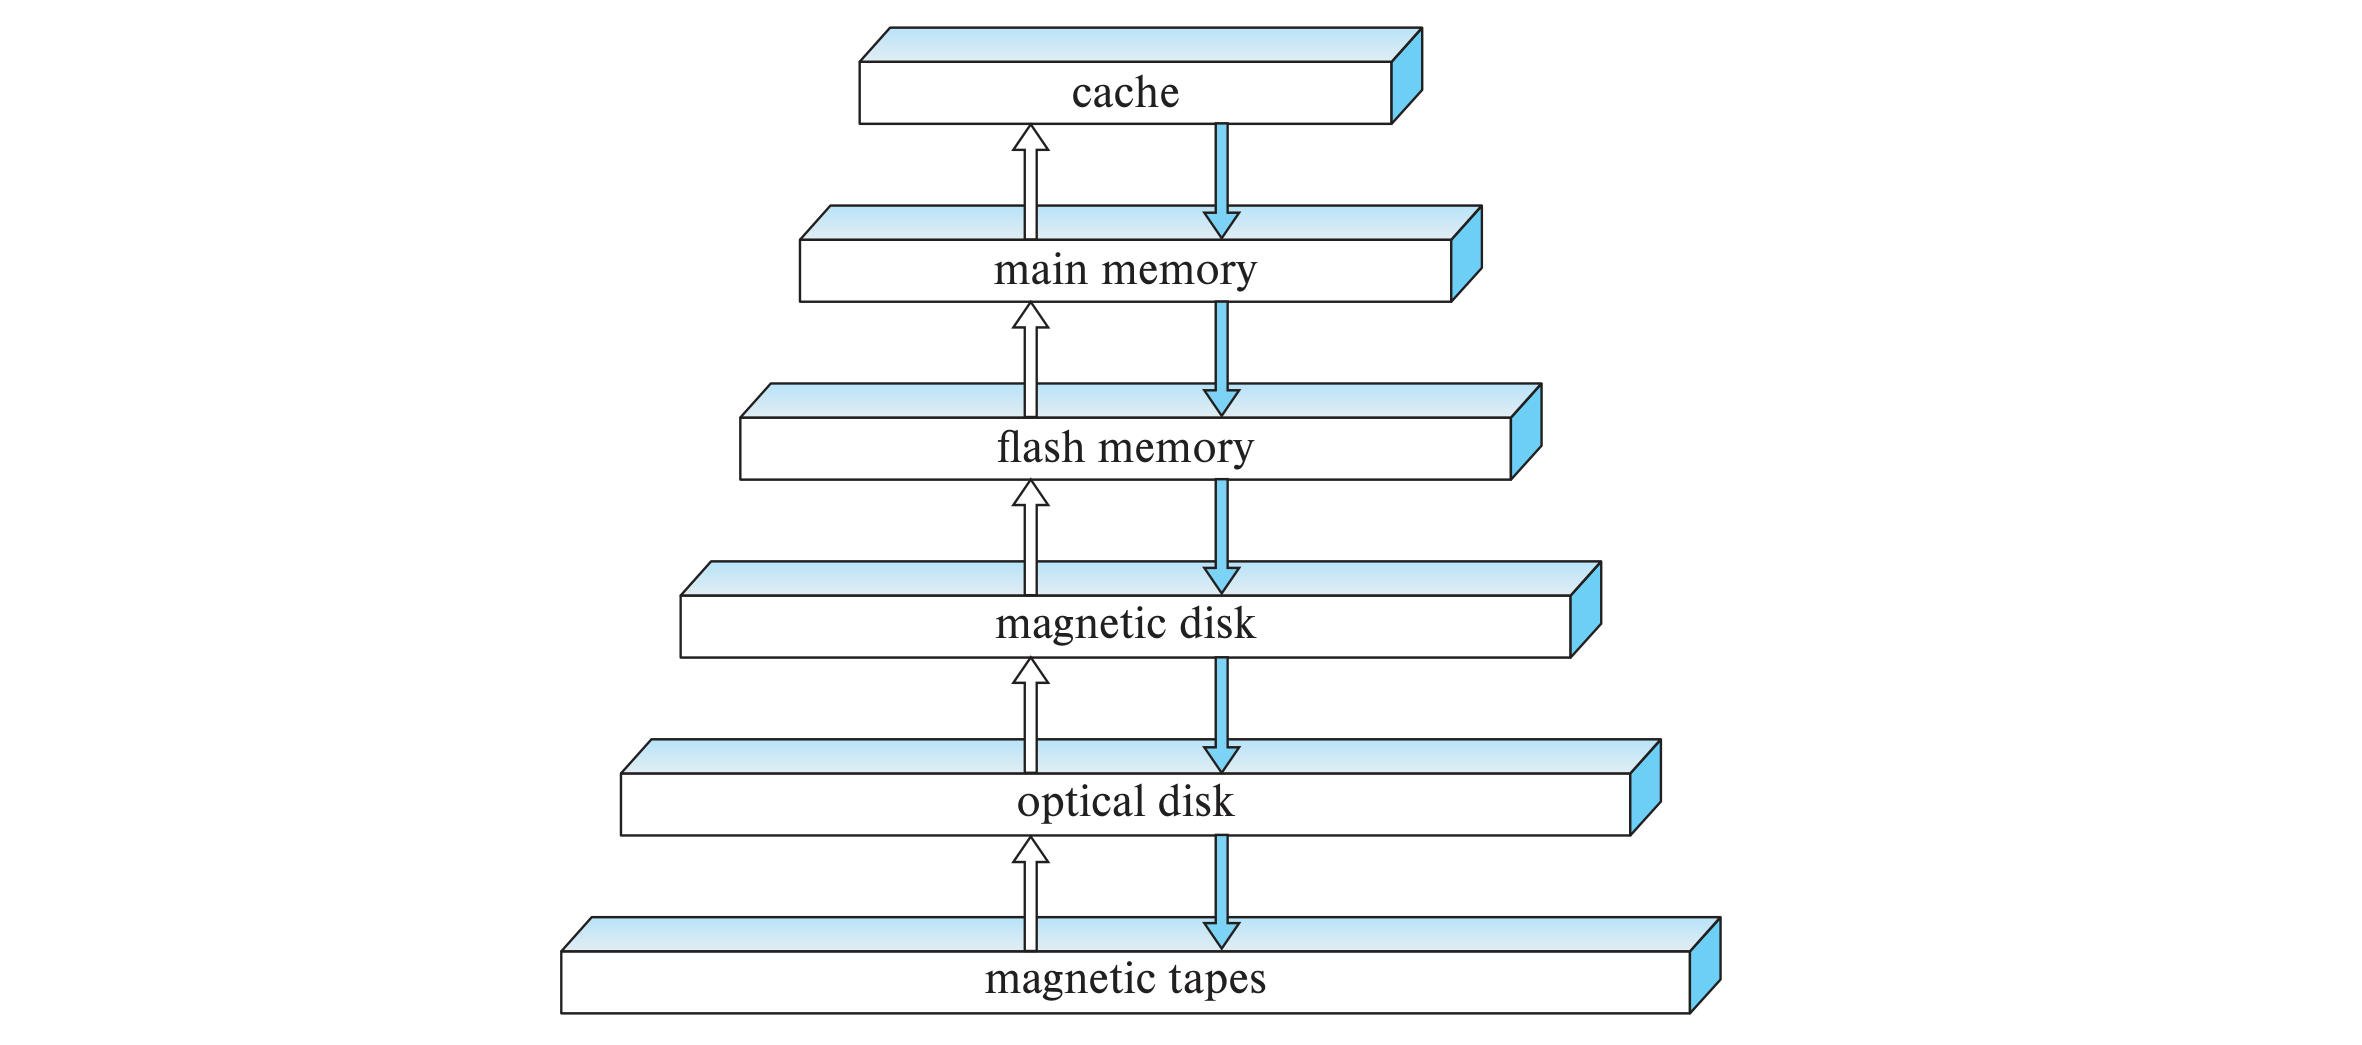
\includegraphics[width=\linewidth]{Figure12.1.png}
    \caption{Storage device hierarchy.}
    \label{Figure:12.1}
\end{figure}

The fastest storage media are referred to as \textcy{primary storage}. The media in the next level in the hierarchy are referred to as \textcy{secondary storage}, or \textcy{online storage}. The media in the lowest level in the hierarchy are referred to as \textcy{tertiary storage}, or \textcy{offline storage}.

\section{Storage Interfaces}

Disks typically support either the \textcy{Serial ATA} (\textcy{SATA}) interface, or the \textcy{Serial Attached SCSI} (\textcy{SAS}) interface; the SAS interface is typically used only in servers. The \textcy{Non-Volatile Memory Express} (\textcy{NVMe}) interface is a logical interface standard developed to better support SSDs and is typically used with the PCIe interface (the PCIe interface provides high-speed data transfer internal to computer systems).

In the \textcy{storage area network} (\textcy{SAN}) architecture, large numbers of disks are connected by a high-speed network to a number of server computers.

\textcy{Network attached storage} (\textcy{NAS}) is an alternative to SAN. Recent years have also seen the growth of \textcy{cloud storage}, where data are stored in the cloud and accessed via an API.

\section{Magnetic Disks}
\subsection{Physical Characteristics of Disks}

Each disk \textcy{platter} has a flat, circular shape. The disk surface is logically divided into \textcy{tracks}, which are subdivided into \textcy{sectors}. A \textcy{sector} is the smallest unit of information that can be read from or written to the disk.

The \textcy{read-write head} stores information on a sector magnetically as reversals of the direction of magnetization of the magnetic material.

A disk typically contains many platters, and the read-write heads of all the tracks are mounted on a single assembly called a \textcy{disk arm} and move together. The disk platters mounted on a spindle and the heads mounted on a disk arm are together known as \textcy{head-disk assemblies}. Since the heads on all the platters move together, when the head on one platter is on the $i$th track, the heads on all other platters are also on the $i$th track of their respective platters. Hence, the $i$th tracks of all the platters together are called the $i$th \textcy{cylinder}.

A \textcy{disk controller} interfaces between the computer system and the actual hardware of the disk drive; in modern disk systems, the disk controller is implemented within the disk drive unit. A disk controller accepts high-level commands to read or write a sector, and initiates actions. Disk controllers also attach \textcy{checksums} to each sector that is written; the checksum is computed from the data written to the sector.

Another interesting task that disk controllers perform is \textcy{remapping of bad sectors}.

\subsection{Performance Measures of Disks}

\textcy{Access time} is the time from when a read or write request is issued to when data transfer begins. The time for repositioning the arm is called the \textcy{seek time}, and it increases with the distance that the arm must move.

The \textcy{average seek time} is the average of the seek times, measured over a sequence of (uniformly distributed) random requests.

Once the head has reached the desired track, the time spent waiting for the sector to be accessed to appear under the head is called the \textcy{rotational latency time}. On an average, one-half of a rotation of the disk is required for the beginning of the desired sector to appear under the head. Thus, the \textcy{average latency time} of the disk is one-half the time for a full rotation of the disk.

The \textcy{data-transfer rate} is the rate at which data can be retrieved from or stored to the disk.

A \textcy{disk block} is a logical unit of storage allocation and retrieval, and block sizes today typically range from 4 to 16 kilobytes. The term \textcy{page} is often used to refer to blocks, although in a few contexts they refer to different things.

In a \textcy{sequential access} pattern, successive requests are for successive block numbers, which are on the same track, or on adjacent tracks.

In contrast, in a \textcy{random access} pattern, successive requests are for blocks that are randomly located on disk. The number of \textcy{I/O operations per second} (\textcy{IOPS}), that is, the number random block accesses that can be satisfied by a disk in a second, depends on the access time, and the block size, and the data transfer rate of the disk.

The final commonly used measure of a disk is the \textcy{mean time to failure} (\textcy{MTTF}),\footnote{The term \textcy{mean time between failures} (\textcy{MTBF}) is often used to refer to MTTF in context of disk drives, although technically MTBF should only be used in the context of systems that can be repaired after failure, and may fail again; MTBF would then be the sum of MTTF and the mean time to repair.} which is a measure of the reliability of the disk.

\section{Flash Memory}

A write to a page of flash memory typically takes about 100 microseconds. However, once written, a page of flash memory cannot be directly overwritten. Instead, it has to be erased and rewritten subsequently. The erase operation must be performed on a group of pages, called an \textcy{erase block}, erasing all the pages in the block, and takes about 2 to 5 milliseconds.

The logical-to-physical page mapping is replicated in an in-memory \textcy{translation table} for quick access.

Since each physical page can be updated only a fixed number of times, physical pages that have been erased many times are assigned "cold data," that is, data that are rarely updated, while pages that have not been erased many times are used to store "hot data," that is, data that are updated frequently. This principle of evenly distributing erase operations across physical blocks is called \textcy{wear leveling} and is usually performed transparently by flash-memory controllers.

All the above actions are carried out by a layer of software called the \textcy{flash translation layer}; above this layer, flash storage looks identical to magnetic disk storage, providing the same page/sector-oriented interface, except that flash storage is much faster.

\begin{framed}
    \begin{center}
        {\textbf{STORAGE CLASS MEMORY}}
    \end{center}

    Although flash is the most widely used type of non-volatile memory, there have been a number of alternative non-volatile memory technologies developed over the years. Several of these technologies allow direct read and write access to individual bytes or words, avoiding the need to read or write in units of pages (and also avoiding the erase overhead of NAND flash). Such types of non-volatile memory are referred to as \textcy{storage class memory}, since they can be treated as a large non-volatile block of memory.
\end{framed}

\textcy{Hybrid disk drives} are hard-disk systems that combine magnetic storage with a smaller amount of flash memory, which is used as a cache for frequently accessed data.

\section{RAID}

A variety of disk-organization techniques, collectively called \textcy{redundant arrays of independent disks} (\textcy{RAID}), have been proposed to achieve improved performance and reliability.

\subsection{Improvement of Reliability via Redundancy}

The solution to the problem of reliability is to introduce \textcy{redundancy}; that is, we store extra information that is not needed normally but that can be used in the event of failure of a disk to rebuild the lost information.

The simplest (but most expensive) approach to introducing redundancy is to duplicate every disk. This technique is called \textcy{mirroring} (or, sometimes, \textit{shadowing}).

The mean time to failure (where failure is the loss of data) of a mirrored disk depends on the mean time to failure of the individual disks, as well as on the \textcy{mean time to repair}, which is the time it takes (on an average) to replace a failed disk and to restore the data on it.

\subsection{Improvement in Performance via Parallelism}

With disk mirroring, the rate at which read requests can be handled is doubled, since read requests can be sent to either disk (as long as both disks in a pair are functional, as is almost always the case). The transfer rate of each read is the same as in a single-disk system, but the number of reads per unit time has doubled.

With multiple disks, we can improve the transfer rate as well (or instead) by \textcy{striping data} across multiple disks. In its simplest form, data striping consists of splitting the bits of each byte across multiple disks; such striping is called \textcy{bit-level striping}.

\textcy{Block-level striping} stripes blocks across multiple disks.

\subsection{RAID Levels}

For a given set of blocks, a \textcy{parity block} can be computed and stored on disk; the $i$th bits of the parity block is computed as the "exclusive or" (XOR) of the $i$th bits of the all blocks in the set.

Whenever a block is written, the parity block for its set must be recomputed and written to disk. The new value of the parity block can be computed by either (i) reading all the other blocks in the set from disk and computing the new parity block, or (ii) by computing the XOR of the old value of the parity block with the old and new value of the updated block. These schemes have different cost-performance trade-offs. The schemes are classified into \textcy{RAID levels}. Figure\;\ref{Figure:12.4} illustrates the four levels that are used in practice. For all levels, the figure depicts four disks’ worth of data, and the extra disks depicted are used to store redundant information for failure recovery.
\begin{itemize}
    \item \textcy{RAID level 0} refers to disk arrays with striping at the level of blocks, but without any redundancy.
    \item \textcy{RAID level 1} refers to disk mirroring with block striping.
    
    Note that some vendors use the term \textcy{RAID level 1+0} or \textcy{RAID level 10} to refer to mirroring with striping, and they use the term RAID level 1 to refer to mirroring without striping.
    \item \textcy{RAID level 5} refers to block-interleaved distributed parity.
    \item \textcy{RAID level 6}, the $P+Q$ redundancy scheme, is much like RAID level 5, but it stores extra redundant information to guard against multiple disk failures.
\end{itemize}

\begin{figure}[htbp]
    \centering
    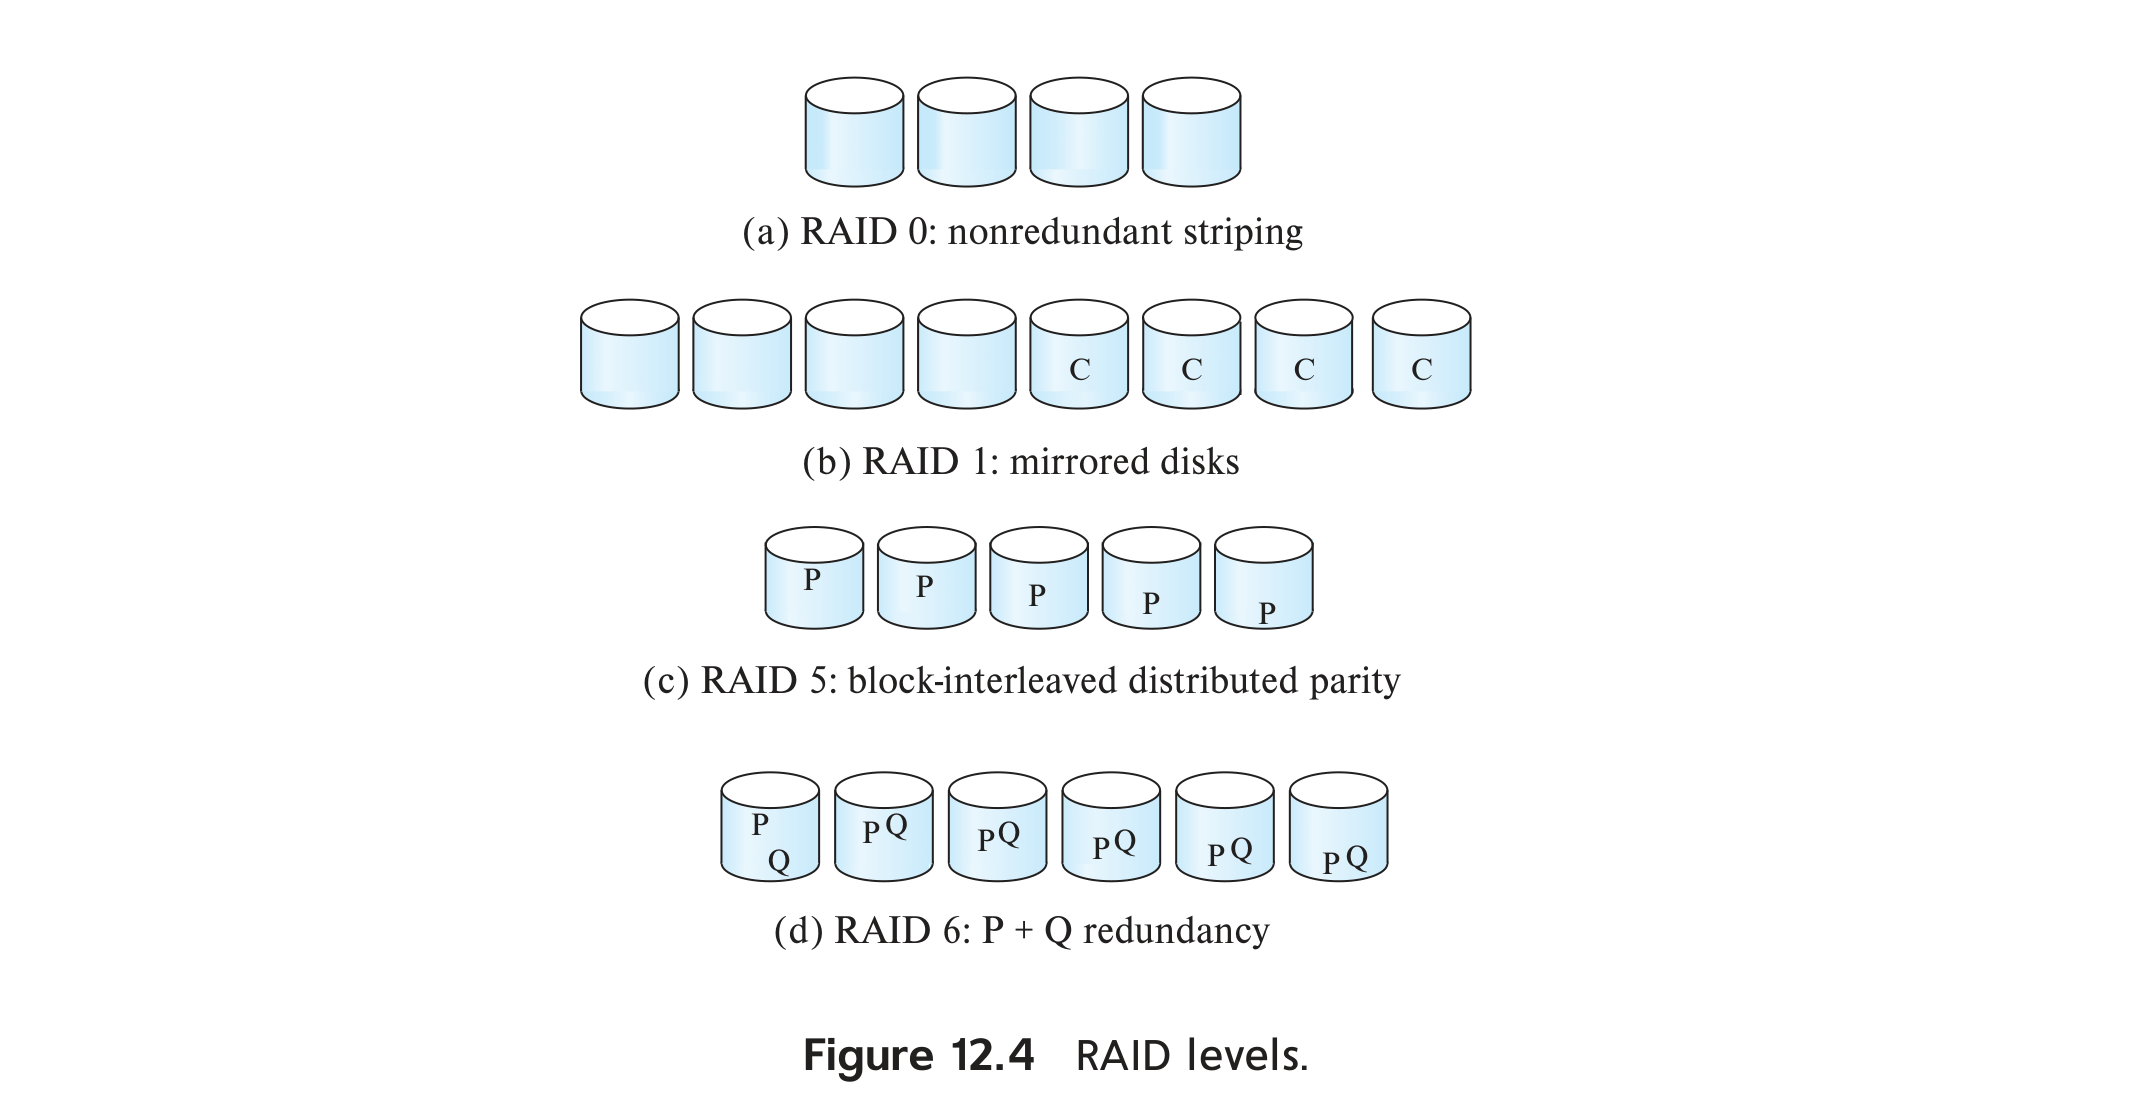
\includegraphics[width=\linewidth]{Figure12.4.png}
    \caption{RAID levels}
    \label{Figure:12.4}
\end{figure}

\subsection{Hardware Issues}

RAID can be implemented with no change at the hardware level, using only software modification. Such RAID implementations are called \textcy{software RAID}. However, there are significant benefits to be had by building special-purpose hardware to support RAID; systems with special hardware support are called \textcy{hardware RAID} systems.

Reasons for loss of data on individual sectors could range from manufacturing defects to data corruption on a track when an adjacent track is written repeatedly. To minimize the chance of such data loss, good RAID controllers perform \textcy{scrubbing}; that is, during periods when disks are idle, every sector of every disk is read, and if any sector is found to be unreadable, the data are recovered from the remaining disks in the RAID organization, and the sector is written back.

Server hardware is often designed to permit \textcy{hot swapping}; that is, faulty disks can be removed and replaced by new ones without turning power off.

\subsection{Choice of RAID Level}

The \textcy{rebuild performance} of a RAID system may be an important factor if continuous availability of data is required, as it is in high-performance database systems.

\section{Disk-Block Access}

Reducing the number of random accesses is very important for data stored on magnetic disks; SSDs support much faster random access than do magnetic disks, so the impact of random access is less with SSDs, but data access from SSDs can still benefit from some of the techniques described below.
\begin{itemize}
    \item \textcy{Buffering}.
    \item \textcy{Read-ahead}. When a disk block is accessed, consecutive blocks from the same track are read into an in-memory buffer even if there is no pending request for the blocks. In the case of sequential access, such \textcy{read-ahead} ensures that many blocks are already in memory when they are requested, and it minimizes the time wasted in disk seeks and rotational latency per block read.
    \item \textcy{Scheduling}. \textcy{Disk-arm-scheduling} algorithms attempt to order accesses to tracks in a fashion that increases the number of accesses that can be processed. A commonly used algorithm is the \textcy{elevator algorithm}, which works in the same way many elevators do.
    \item \textcy{File organization}.
    
    Storing a large file in a single long sequence of consecutive blocks poses challenges to disk block allocation; instead, operating systems allocate some number of consecutive blocks (an \textcy{extent}) at a time to a file.

    Over time, a sequential file that has multiple small appends may become \textcy{fragmented}; that is, its blocks become scattered all over the disk.
    \item \textcy{Non-volatile write buffers}.
    
    We can use \textit{non-volatile random-access memory} (NVRAM) to speed up disk writes. The idea is that, when the database system (or the operating system) requests that a block be written to disk, the disk controller writes the block to a \textcy{non-volatile write buffer} and immediately notifies the operating system that the write completed successfully. 
\end{itemize}

\chapter{Data Storage Structures}
\section{Database Storage Architecture}

Databases that store the entire database in memory and optimize in-memory data structures as well as query processing and other algorithms used by the database to exploit the memory residency of data are called \textcy{main-memory databases}.

\section{File Organization}

A \textcy{file} is organized logically as a sequence of records.

Each file is also logically partitioned into fixed-length storage units called \textcy{blocks}, which are the units of both storage allocation and data transfer.

\subsection{Fixed-Length Records}

At the beginning of the file, we allocate a certain number of bytes as a \textcy{file header}. The header will contain a variety of information about the file. For now, all we need to store there is the address of the first record whose contents are deleted. We use this first record to store the address of the second available record, and so on. The deleted records thus form a linked list, which is often referred to as a \textcy{free list}.

\subsection{Variable-Length Records}

\textcy{Variable-length records} arise in database systems due to several reasons.

The \textcy{slotted-page structure} is commonly used for organizing records within a block.

\subsection{Storing Large Objects}

\textcy{Large objects} may be stored either as files in file system area managed by the database, or as file structures stored in and managed by the database.

\section{Organization of Records in Files}

Several of the possible ways of organizing records in files are:
\begin{itemize}
    \item \textcy{Heap file organization}.
    \item \textcy{Sequential file organization}.
    \item \textcy{Multitable clustering file organization}: Generally, a separate file or set of files is used to store the records of each relation.
    \item \textcy{B+-tree file organization}.
    \item \textcy{Hashing file organization}.
\end{itemize}

\subsection{Heap File Organization}

Most databases use a space-efficient data structure called a \textcy{free-space map} to track which blocks have free space to store records.

\subsection{Sequential File Organization}

A \textcy{sequential file} is designed for efficient processing of records in sorted order based on some search key. A \textcy{search key} is any attribute or set attributes; it need not be the primary key, or even a superkey.

We can manage deletion by using pointer chains. For insertion, we apply the following two rules:
\begin{enumerate}
    \item Locate the record in the file that comes before the record to be inserted in search-key order.
    \item If there is a free record (i.e., space left after a deletion) within the same block as this record, insert the new record there. Otherwise, insert the new record in an \textit{overflow block}. In either case, adjust the pointers so as to chain together the records in search-key order. 
\end{enumerate}

If relatively few records need to be stored in overflow blocks, this approach works well. Eventually, however, the correspondence between search-key order and physical order may be totally lost over a period of time, in which case sequential processing will become much less efficient. At this point, the file should be \textcy{reorganized} so that it is once again physically in sequential order.

\subsection{Multitable Clustering File Organization}

A \textcy{multitable clustering file organization} is a file organization that stores related records of two or more relations in each block. The \textcy{cluster key} is the attribute that defines which records are stored together.

\subsection{Partitioning}

Many databases allow the records in a relation to be partitioned into smaller relations that are stored separately. Such \textcy{table partitioning} is typically done on the basis of an attribute value.

\section{Data-Dictionary Storage}

A relational database system needs to maintain data \textit{about} the relations. In general, such "data about data" are referred to as \textcy{metadata}.

Relational schemas and other metadata about relations are stored in a structure called the \textcy{data dictionary} or \textcy{system catalog}.

\section{Database Buffer}

The \textcy{buffer} is that part of main memory available for storage of copies of disk blocks. The subsystem responsible for the allocation of buffer space is called the \textcy{buffer manager}.

\subsection{Buffer Manager}
\subsubsection{Buffer replacement strategy}

When there is no room left in the buffer, a block must be \textcy{evicted}, that is, removed, from the buffer before a new one can be read in. Most operating systems use a \textcy{least recently used} (\textcy{LRU}) scheme, in which the block that was referenced least recently is written back to disk and is removed from the buffer.

\subsubsection{Pinned blocks}

Once a block has been brought into the buffer, a database process can read the contents of the block from the buffer memory.

It is therefore important that before a process reads data from a buffer block, it ensures that the block will not get evicted. To do so, the process executes a \textcy{pin} operation on the block; the buffer manager never evicts a pinned block. When it has finished reading data, the process should execute an \textcy{unpin} operation, allowing the block to be evicted when required.

Multiple processes can read data from a block that is in the buffer. The block cannot be evicted until all processes that have executed a pin have then executed an unpin operation. A simple way to ensure this property is to keep a \textcy{pin count} for each buffer block.

\subsubsection{Forced output of blocks}

There are situations in which it is necessary to write a block to disk, to ensure that certain data on disk are in a consistent state. Such a write is called a \textcy{forced output} of a block.

\section{Buffer-Replacement Strategies}

The assumption generally made is that blocks that have been referenced recently are likely to be referenced again. Therefore, if a block must be replaced, the least recently referenced block is replaced. This approach is called the \textcy{least recently used} (\textcy{LRU}) block-replacement scheme.

\subsection{Reordering of Writes and Recovery}

If a non-volatile write buffer were available, it could be used to perform the writes in order to non-volatile RAM and later reorder the writes when writing them to disk.

However, most disks do not come with a non-volatile write buffer; instead, modern file systems assign a disk for storing a log of the writes in the order that they are performed. Such a disk is called a \textcy{log disk}.

File systems that support log disks as above are called \textcy{journaling file systems}.

\section{Column-Oriented Storage}

Databases traditionally store all attributes of a tuple together in a record, and tuples are stored in a file. Such a storage layout is referred to as a \textit{row-oriented storage}.

In contrast, in \textcy{column-oriented storage}, also called a \textcy{columnar storage}, each attribute of a relation is stored separately with values of the attribute from successive tuples stored at successive positions in the file.

If a query needs to access the entire contents of the $i$th row of a table, the values at the $i$th position in each of the columns are retrieved and used to reconstruct the row. Column-oriented storage thus has the drawback that fetching multiple attributes of a single tuple requires multiple I/O operations. Thus, it is not suitable for queries that fetch multiple attributes from a few rows of a relation.

However, column-oriented storage is well suited for data analysis queries, which process many rows of a relation, but often only access some of the attributes. The reasons are as follows:
\begin{itemize}
    \item \textbf{Reduced I/O}.
    \item \textbf{Improved CPU cache performance}.
    \item \textbf{Improved compression}.
    \item \textbf{vector processing}. Many modern CPU architectures support \textcy{vector processing}, which allows a CPU operation to be applied in parallel on a number of elements of an array.
\end{itemize}

Databases that use column-oriented storage are referred to as \textcy{column stores}, while databases that use row-oriented storage are referred to as \textcy{row stores}.

In ORC, a row-oriented representation is converted to column-oriented representation as follows: A sequence of tuples occupying several hundred megabytes is broken up into a columnar representation called a \textcy{stripe}.

Some databases support two underlying storage systems, one a row-oriented one designed for transaction processing, and the second a column-oriented one, designed for data analysis. Such systems are called \textcy{hybrid row/column stores}.

\section{Storage Organization in Main-Memory Databases}

A \textcy{main-memory database} is a database where all data reside in memory; main-memory database systems are typically designed to optimize performance by making use of this fact.

\chapter{Indexing}
\section{Basic Concepts}

We shall consider several techniques for ordered indexing. Each technique must be evaluated on the basis of these factors:
\begin{itemize}
    \item \textcy{Access types}: The types of access that are supported efficiently.
    \item \textcy{Access time}: The time it takes to find a particular data item, or set of items, using the technique in question.
    \item \textcy{Insertion time}: The time it takes to insert a new data item.
    \item \textcy{Deletion time}: The time it takes to delete a date item.
    \item \textcy{Space overhead}: The additional space occupied by an index structure.
\end{itemize}

An attribute or set of attributes used to look up records in a file is called a \textcy{search key}.

\section{Ordered Indices}

An \textcy{ordered index} stores the values of the search keys in sorted order and associates with each search key the records that contain it.

If the file containing the records is sequentially ordered, a \textcy{clustering index} is an index whose search key also defines the sequential order of the file. Clustering indices are also called \textcy{primary indices}; the term \textit{primary index} may appear to denote an index on a primary key, but such indices can in fact be built on any search key. Indices whose search key specifies an order different from the sequential order of the file are called \textcy{nonclustering indices}, or \textcy{secondary indices}.

Such files, with a clustering index on the search key, are called \textcy{index-sequential files}.

\subsection{Dense and Sparse Indices}

An \textcy{index entry}, or \textcy{index record}, consists of a search-key value and pointers to one or more records with that value as their search-key value.

There are two types of ordered indices that we can use:
\begin{itemize}
    \item \textcy{Dense index}: In a dense index, an index entry appears for every search-key value in the file.
    \item \textcy{Sparse index}: In a sparse index, an index entry appears for only some of the search-key values.
\end{itemize}

\subsection{Multilevel Indices}

Indices with two or more levels are called \textcy{multilevel indices}.

\subsection{Secondary Indices}

If a relation can have more than one record containing the same search key value (that is, two or more records can have the same values for the indexed attributes), the search key is said to be a \textcy{nonunique search key}.

\subsection{Indices on Multiple Keys}

A search key containing more than one attribute is referred to as a \textcy{composite search key}.

\section{B$^+$-Tree Index Files}

The \textcy{B$^+$-tree index} structure is most widely used of several index structures that maintain their efficiency despite insertion and deletion of data. A B$^+$-tree index takes the form of a \textcy{balanced tree} in which every path from the root of the tree to a leaf of the tree is of the same length.

\subsection{Structure of a B$^+$-Tree}

We consider first the structure of the \textcy{leaf nodes}.

The \textcy{nonleaf nodes} of the B$^+$-tree form a multilevel (sparse) index on the leaf nodes. Nonleaf nodes are also referred to as \textcy{internal nodes}.

\subsection{Queries on B$^+$-Trees}

Let us consider how we process queries on a B$^+$-tree.

B$^+$-tree can also be used to find all records with search key values in a specified range $[lb,ub]$. Such queries are called \textcy{range queries}.

\subsection{Updates on B$^+$-Trees}

Insertion and deletion are more complicated than lookup, since it may be necessary to \textcy{split} a node that becomes too large as the result of an insertion, or to \textcy{coalesce} nodes (i.e., combine nodes) if a node becomes too small (fewer than $\lceil n/2\rceil$ pointers).

\subsection{Nonunique Search Keys}

We have assumed so far that search keys are unique. Recall also how to make search keys unique by creating a composite search key containing the original search key and extra attributes, that together are unique across all records.

The extra attribute is called a \textcy{uniquifier} attribute.

\section{B$^+$-Tree Extensions}
\subsection{B$^+$-Tree File Organization}

In a \textcy{B$^+$-tree file organization}, the leaf nodes of the tree store records, instead of storing pointers to records.

\subsection{Indexing Strings}

The fanout of nodes can be increased by using a technique called \textcy{prefix compression}.

\subsection{Bulk Loading of B$^+$-Tree Indices}

Insertion of a large number of entries at a time into an index is referred to as \textcy{bulk loading} of the index.

In \textcy{bottom-up B$^+$-tree construction}, after sorting the entries, we break up the sorted entries into blocks, keeping as many entries in a block as can fit in the block; the resulting blocks form the leaf level of the B$^+$-tree.

\subsection{B-Tree Index Files}

\textcy{B-tree indices} are similar to B$^+$-tree indices.

\section{Hash Indices}

In our description of hashing, we shall use the term \textcy{bucket} to denote a unit of storage that can store one or more records. In a \textcy{hash file organization}, instead of record pointers, buckets store the actual records; such structures only make sense with disk-resident data.

Formally, let $K$ denote the set of all search-key values, and let $B$ denote the set of all bucket addresses. A \textcy{hash function} $h$ is a function from $K$ to $B$.

To insert a record with search key $K_i$, we compute $h(K_i)$, which gives the address of the bucket for that record. We add the index entry for the record to the list at offset $i$. Note that there are other variants of hash indices that handle the case of multiple records in a bucket differently; the form described here is the most widely used variant and is called \textcy{overflow chaining}.

Hash indexing using overflow chaining is also called \textcy{closed addressing} (or, less commonly, \textcy{closed hashing}).

In a disk-based hash index, when we insert a record, we locate the bucket by using hashing on the search key, as described earlier. Assume for now that there is space in the bucket to store the record. Then, the record is stored in that bucket. If the bucket does not have enough space, a \textcy{bucket overflow} is said to occur. We handle bucket overflow by using \textcy{overflow buckets}.

Bucket overflow can occur if there are insufficient buckets for the given number of records. Bucket overflow can also occur if some buckets are assigned more records than are others, resulting in one bucket overflowing even when other buckets still have a lot of free space.

Such \textcy{skew} in the distribution of records can occur if multiple records may have the same search key.

Hash indexing where the number of buckets is fixed when the index is created, is called \textcy{static hashing}. One of the problems with static hashing is that we need to know how many records are going to be stored in the index.

To handle this problem, the hash index can be rebuilt with an increased number of buckets. For example, if the number of records becomes twice the number of buckets, the index can be rebuilt with twice as many buckets as before. However, rebuilding the index has the drawback that it can take a long time if the relations are large, causing disruption of normal processing. Several schemes have been proposed that allow the number of buckets to be increased in a more incremental fashion. Such schemes are called \textcy{dynamic hashing} techniques; the \textit{linear hashing} technique and the \textit{extendable hashing} technique are two such schemes.

\section{Multiple-Key Access}
\subsection{Covering Indices}

\textcy{Covering indices} are indices that store the values of some attributes (other than the search-key attributes) along with the pointers to the record.

\section{Write-Optimized Index Structures}

The \textcy{log-structured merge tree} or LSM tree and its variants are write-optimized index structures that have seen very significant adoption.

\subsection{LSM Trees}

An LSM tree consists of several B$^+$-trees, starting with an in-memory tree, called $L_0$, and on-disk trees $L_1,L_2,\ldots,L_k$ for some $k$, where $k$ is called the level.

Note that all entries in the leaf level of the old $L_1$ tree, including those in leaf nodes that do not have any updates, are copied to the new tree instead of performing updates on the existing $L_1$ tree node. This gives the following benefits:
\begin{enumerate}
    \item The leaves of the new tree are sequentially located, avoiding random $I/O$ during subsequent merges.
    \item The leaves are full, avoiding the overhead of partially occupied leaves that can occur with page splits.
\end{enumerate}
There is, however, a cost to using the LSM structure as described above: the entire contents of the tree are copied each time a set of entries from $L_0$ are copied into $L_1$. One of two techniques is used to reduce this cost:
\begin{itemize}
    \item Multiple levels are used, with level $L_{i+1}$ trees having a maximum size that is $k$ times the maximum size of level $L_i$ trees.
    \item Each level (other than $L_0$) can have up to some number $b$ of trees, instead of just 1 tree.
    
    This variant of the LSM tree is called a \textcy{stepped-merge index}.
\end{itemize}

Instead of directly finding an index entry and deleting it, deletion results in insertion of a new \textcy{deletion entry} that indicates which index entry is to be deleted.

\subsection{Buffer Tree}

The key idea behind the \textcy{buffer tree} is to associate a buffer with each internal node of a B$^+$-tree, including the root node.

Buffer trees have been implemented as part of the \textcy{Generalized Search Tree} (\textcy{GiST}) index structure in PostgreSQL.

\section{Bitmap Indices}

A \textcy{bitmap} is simply an array of bits. In it simplest form, a \textcy{bitmap index} on the attribute $A$ of relation $r$ consists of one bitmap for each value that $A$ can take.

\section{Indexing of Spatial and Temporal Data}
\subsection{Indexing of Spatial Data}

A tree structure called a \textcy{k-d tree} was one of the early structures used for indexing in multiple dimensions.

The \textcy{k-d-B tree} extends the k-d tree to allow multiple child nodes for each internal node, just as a B-tree extends a binary tree, to reduce the height of the tree.

Instead of dividing the data one dimension at a time, \textcy{quadtrees} divide up a two-dimensional space into four quadrants at each node of the tree.

A storage structure called an \textcy{R-tree} is useful for indexing of objects spanning regions of space in addition to points. An R-tree is a balanced tree structure with the indexed objects stored in leaf nodes. However, instead of a range of values, a rectangular \textcy{bounding box} is associated with each tree node.

\subsection{Indexing Temporal Data}

A \textcy{time interval} has a start time and an end time. Further a time interval indicates whether the interval starts at the start time, or just after the start time, that is, whether the interval is \textcy{closed} or \textcy{open} at the start time.

% %--------------------------------------------------------------------------
% %         Bibliographie 
% %--------------------------------------------------------------------------
\end{document}